\section{Work and Power}

\underline{\textbf{Part 1}} \par
Use a constant horizontal force to push a block ($v_i = 0$) up a ramp that has friction.
Choose and record all relevant values.
Identify all forces present, label each one as conservative or non-conservative, and calculate the amount of work each one does on the block.
Use these work values to calculate the expected final velocity after some time interval.
Compare this calculation to the final velocity measured by IP.

\begin{figure}[H]
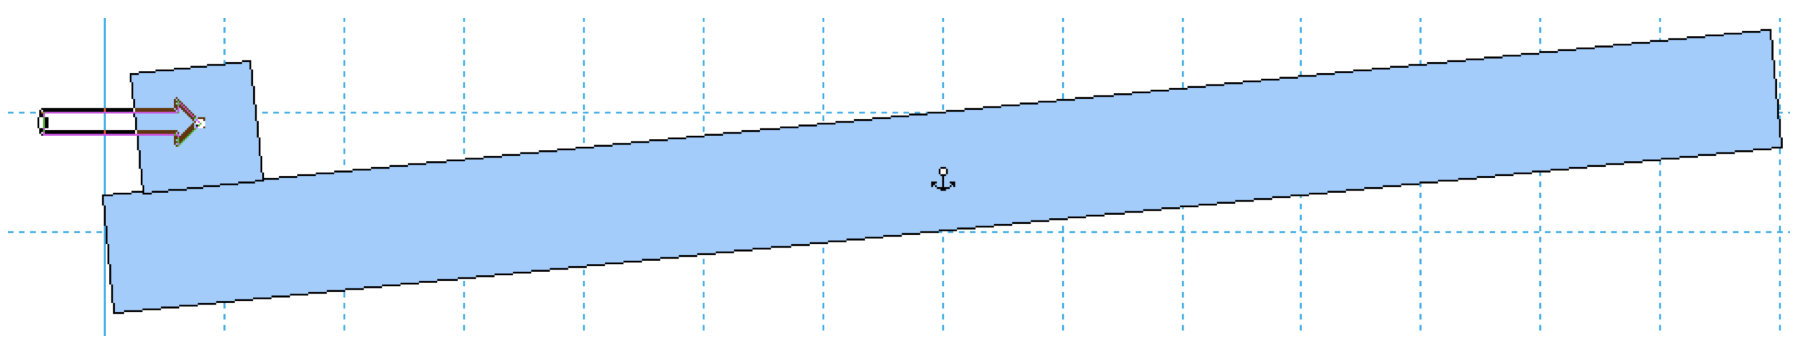
\includegraphics[scale=0.50]{figures/workPower/fig1.png}
\end{figure}


\underline{\textbf{Part 2}} \par
In this lab you will conduct a real life experiment to calculate your (or a lab mate's) maximum power output, with an uncertainty.

\begin{enumerate}
\item Write down your weight (with uncertainty) and convert to mass (in kg).
\item Gather relevant supplies (a ruler, stopwatch/smartphone, paper, pencil, and calculator) and go as a class to the staircase next to the Nesbitt building.
\item Use your ruler to measure the height of one stair. Also count the number of stairs to get the total elevation change from the bottom to the top. Make sure to propagate the error.
\item Have one person control the stop watch while another person runs up the hill next to the staircase as fast as possible. Record the time taken, with uncertainty. The runner and timer should coordinate a strategy so that the runner's velocity at the bottom is approximately equal to the velocity at the top; that way the change in energy is only due to the change in height. Include your strategy in your lab report. Although your stopwatch probably has very good precision, you may want to assign a larger time uncertainty due to the human error of starting and stopping at the right time.
\item Write down the relevant equations from class and calculate your power with uncertainty. Give your answer both in W and hp.
\end{enumerate}

\pagebreak \clearpage
